\subsection{Audio In/Out Port}

The {\it \systemNameFull} includes an audio port that is connected to the audio CODEC
(COder/DECoder) chip on the \DEBoard~board. The default setting for the 
sample rate provided by the audio CODEC is 
8K samples/sec.  The audio port provides audio-input capability via the microphone 
jack on the \DEBoard~board, as well as audio output functionality via the line-out jack.  
The audio port includes four FIFOs that are used to hold incoming and outgoing data.
Incoming data is stored in the left- and right-channel {\it Read} FIFOs, and outgoing data
is held in the left- and right-channel {\it Write} FIFOs. All FIFOs have a maximum 
depth of 128 32-bit words.

The audio port's programming interface consists of four 32-bit registers, as illustrated in 
Figure \ref{fig:audio_port}.  The {\it Control} register, which has the address 
{\sf 0xFF203040}, is readable to provide status information and writable to make control
settings. Bit {\it RE} of this register provides an interrupt enable capability for
incoming data. Setting this bit to 1 allows the audio core to generate a \processor~interrupt
when either of the {\it Read} FIFOs are filled 75\% or more. The bit {\it RI} will then be
set to 1 to indicate that the interrupt is pending. The interrupt can be cleared by removing
data from the {\it Read} FIFOs until both are less than 75\% full. 
Bit {\it WE} gives an interrupt enable capability for outgoing data. Setting this bit to 
1 allows the audio core to generate an interrupt when either of the {\it Write} FIFOs are
less that 25\% full. The bit {\it WI} will be set to 1 to indicate that the interrupt 
is pending, and it can be cleared by filling the {\it Write} FIFOs until both 
are more than 25\% full.  The bits {\it CR} and {\it CW} in Figure \ref{fig:audio_port} can 
be set to 1 to clear the {\it Read} and {\it Write} FIFOs, respectively. The clear function 
remains active until the corresponding bit is set back to 0.

\begin{figure}[h!]
   \begin{center}
       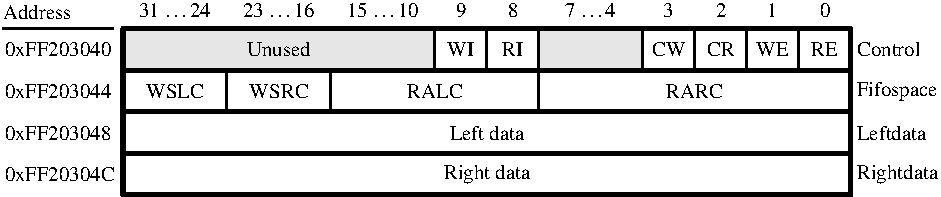
\includegraphics{../../../common/figs/Media_FPGA_Audio_Address_Map.pdf}
   \end{center}
   \caption{Audio port registers.}
	\label{fig:audio_port}
\end{figure}

The read-only {\it Fifospace} register in Figure \ref{fig:audio_port} contains four 8-bit fields.
The fields {\it RARC} and {\it RALC} give the number of words currently stored in the 
right and left audio-input FIFOs, respectively. The fields {\it WSRC} and {\it WSLC} give 
the number of words currently available (that is, {\it unused}) for storing data in the right 
and left audio-out FIFOs. When all FIFOs in the audio port are cleared, the values provided 
in the {\it Fifospace} register are {\it RARC} $=$ {\it RALC} $=$ 0 
and {\it WSRC} $=$ {\it WSLC} $=$ 128.

The {\it Leftdata} and {\it Rightdata} registers are readable for audio in, and writable
for audio out. When data is read from these registers, it is provided from the head of the
{\it Read} FIFOs, and when data is written into these registers it is loaded into the {\it
Write} FIFOs.

A fragment of C code that uses the audio port is shown in Listing \ref{lst:audio_example_C}.
The code checks to
see when the depth of either the left or right {\it Read} FIFO has exceeded 75\% full, and then
moves the data from these FIFOs into a memory buffer. This code is part of a program
that is distributed as part of the \productNameMed{}. The source code can be 
found under the heading {\it sample programs}, and is identified by the name 
{\it Audio}.



